\documentclass[tikz]{standalone}
\usepackage{amsmath}
\usetikzlibrary{calc}
\begin{document}
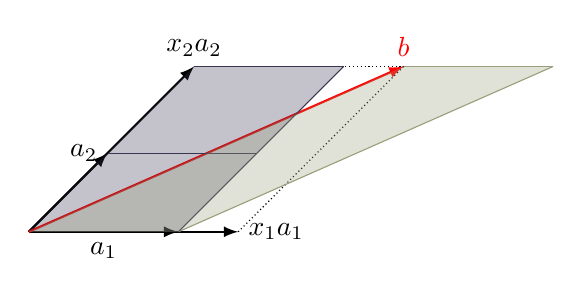
\begin{tikzpicture}[scale=1.0]
\definecolor{la_white}{RGB}{233,235,223} %#E9EBDF
\definecolor{la_dark}{RGB}{59,54,81}     %#3B3651
\definecolor{la_gray}{RGB}{96,112,139}   %#60708B
\definecolor{la_tan}{RGB}{152,159,122}   %#989F7A

\def\xa{1.4}
\def\xb{2.1}
\def\aax{1.9}
\def\abx{1}
\def\aby{1}

\coordinate (O)  at (0,0);
\coordinate (AA) at (\aax,0);
\coordinate (AB) at (\abx,\aby);

\coordinate (AAX) at ({\xa*\aax},0);
\coordinate (ABX) at ({\xb*\abx},{\xb*\aby});
\coordinate (S)   at ({\xb*\abx+\aax},{\xb*\aby});
\coordinate (SX)   at ({\abx+\aax},{\aby});

\coordinate (B) at ({\xa*\aax+\xb*\abx},{\xb*\aby});
\coordinate (D) at ({\xa*\aax+\xb*\abx+\aax},{\xb*\aby});

\draw [densely dotted,black] (ABX) -- (D) ;
\draw [densely dotted,black] (AAX) -- (B) ;
\draw [->,-latex,thick,black] (O) -- (ABX) node [above,pos=1]{$x_2 a_2$};
\draw [->,-latex,thick,black] (O) -- (AAX) node [right,pos=1]{$x_1 a_1$};
\draw [->,-latex,thick,black] (O) -- (AA) node [below,pos=.5]{$a_1$};
\draw [->,-latex,thick,black] (O) -- (AB) node [left,pos=1]{$a_2$};
\draw [->,-latex,thick,red] (O) -- (B) node [above,pos=1]{$b$};
\draw [la_tan] (AA) -- (D) ;
\draw [la_tan] (B) -- (D) ;
\draw [la_dark] (AA) -- (S) ;
\draw [la_dark] (ABX) -- (S) ;
\draw [la_dark] (AB) -- (SX) ;

\fill [la_dark,opacity=0.3] (O) -- (AA) -- (S) -- (ABX) -- cycle;
\fill [la_tan,opacity=0.3] (O) -- (AA) -- (D) -- (B) -- cycle;

\end{tikzpicture}
\end{document}